\section[冲量]{\makebox[5em][s]{冲量}}\label{sec:08.02}

体系能量的变化用外力作的功来描写,体系的动量的变化用
什么来描写?这就是本节将要讨论的问题。

根据牛顿第二定律,对于单个质点有
\begin{equation*}
  m \frac { \dif \vec{v} } { \dif t } = \vec{F}
\end{equation*}
因单个质点的动量为$ \vec{P} = m \vec{v} $,故上述方程可写为
\begin{equation}\label{eqn:08.02.01}
  \frac { \dif \vec{P} } { \dif t } = \vec{F}
\end{equation}
即质点动量的变化率等于外力。

若质点在$ t _ { 1 } $时,具有动量$\vec{P} _ 1$;在$ t _ { 2 } $时,变到$\vec{P} _ 2$,则由式 \eqref{eqn:08.02.01}
得
\begin{equation}\label{eqn:08.02.02}
  \vec{P} _ { 2 } - \vec{P} _ { 1 } = \int _ { t _ { 1 } } ^ { t _ { 2 } } \vec{F} \dif t
\end{equation}
即质点动量的变化,等于力对时间的积分。

$ \displaystyle \int _ { t _ { 1 } } ^ { t _ { 2 } } \vec{F} \dif t $
称为冲量。如果力为常量,则在$ t_1 $到$ t_2 $间的冲量可
写为$ \vec{F} \left( t _ { 2 } - t _ { 1 } \right) $。所以,冲量就是度量动量变化的物理量。

% 233.jpg
\clearpage
比较式\eqref{eqn:08.02.02}与式\eqref{eqn:06.02.08}\lhbrak 考虑到式\eqref{eqn:06.02.01}\rhbrak ,两者在形式
上是非常相似的,前者是力对时间的积分,后者是力对空间的积
分;前者反映出力与时间的联系,后者反映出力与空间的联系。
由此也可看到动量守恒与能量守恒二者的相同与不同。

作为动量守恒定律的一个应用,我们来讨论航天飞船问题。
飞船之所以能上天,是依靠火箭喷出气体的推动力。现在我们来
计算为要达到某一速度需要多少燃料的问题。乍看起来,这似乎
是个与燃料化学性质等有关的复杂问题,实际上,根据动量守恒,
可以给出一个基本关系。因为在应用动量守恒定律时,根本不需
顾及力的具体性质。

% TODO: \usepackage{graphicx} required
\begin{figure}[h]
  \centering
  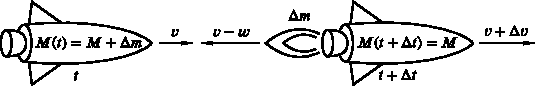
\includegraphics{figure/fig08.04}
  \caption{飞船的运动}
  \label{fig:08.04}
\end{figure}

如图\ref{fig:08.04}所示,在$ t $时刻,飞船的质量为$ M \left( t \right) = M + \Delta m $,速
度为$ v $;在$ t + \Delta t $时刻,喷出质量$ \Delta m $,飞船质量变为$ M \left( t + \Delta t \right) = M $,
速度变为$ v + \Delta v $,如果喷出质量相对主体的速度为$ w $,则喷出质
量相对于地面的速度是$ \left( v - w \right) $。我们可以把它们看作两个质点构
成的孤立体系(忽略重力等其他作用),根据动量守恒,有
\begin{equation*}
  \begin{split}
    & \left( M + \Delta m \right) v \\
    = & \Delta m \left( v - w \right) + M \left( v + \Delta v \right)
  \end{split}
\end{equation*}
整理后得
\begin{equation}\label{eqn:08.02.03}
  \Delta m w = M \Delta v
\end{equation}
两边除以$ \Delta t $后,得
\begin{equation*}
  w \frac { \Delta m } { \Delta t } = M \frac { \Delta v } { \Delta t }
\end{equation*}
在$ \Delta t \to 0 $的极限情况,上式成为

% 234.jpg
\mbox{}\vspace{-1.5em}
\begin{equation}\label{eqn:08.02.04}
  w \frac { \dif m } { \dif t } = M \frac { \dif v } { \dif t }
\end{equation}
这就是飞船所要满足的动力学方程,$ \dfrac { \Delta m } { \dif t } $
是单位时间内所喷出
燃料的质量。

我们还可以进一步改写式\eqref{eqn:08.02.04},因为
\begin{equation*}
  \begin{split}
    \Delta m & = M \left( t \right) - M \left( t + \Delta t \right) \\
    & = - \Delta M
  \end{split}
\end{equation*}
故由式\eqref{eqn:08.02.03},得
\begin{equation*}
  \begin{split}
    \Delta v &= w \frac { \Delta m } { M } \\
    & = - w \frac { \Delta M } { M }
  \end{split}
\end{equation*}
写成微分关系,则有
\begin{equation*}
  \dif v = - w \frac { \dif M } { M }
\end{equation*}
积分后,得到
\begin{equation*}
  \begin{split}
    v _ { 2 } - v _ { 1 } & = - w \int _ { M _ { 1 } } ^ { M ^ { 2 } } \frac { \dif M } { M } \\
    & = w \ln \frac { M _ { 1 } } { M _ { 2 } }
  \end{split}
\end{equation*}

如果开始时,飞船速度$ v _ { 1 } = 0 $,质量$ M _ { 1 } = M _ { \text { 总 } } = M _ { \text { 船 } } + M _ { \text { 燃料 } } $,燃料燃烧完时,飞船达到的速度为$ v _ { 2 } = v $,质量为$ M _ { 2 } = M _ { \text { 船 } } $,则
\begin{equation}\label{key}
  \begin{split}
    v & = w \ln \frac { M _ { \text { 总 } } } { M _ { \text { 船 } } } \\
    & = w \ln \left( \frac { M _ { \text { 船 } } + M _ { \text { 燃料 } } } { M _ { \text { 船 } } } \right) \\
    & = w \ln \left( 1 + \frac { M _ { \text { 燃料 } } } { M _ { \text { 船 } } } \right)
  \end{split}
\end{equation}
% 235.jpg

这就是我们所需要的一般关系。它告诉我们燃料的质量、飞
的质量、气体的喷出速度与飞船所能达到的速度之间的关系。
